\section{V8 JavaScript Engine Pipeline}
\frame{\sectionpage}

\begin{frame}{How does V8 work?}
    \begin{block}{V8 is a JIT Compiler for JavaScript and WebAssembly}
    JIT compilers are compilers that profile code as it runs, generating optimizations along the way for ``hot" code, or code that runs many times. 
    \end{block}
    \begin{block}{Simplified V8 Pipeline}
        \begin{enumerate}
            \item Parser -- Generate an AST from the JavaScript code
            \item Interpreter -- Named ``Ignition", generates an IL representation called Ignition bytecode
            \item Early Compiler -- Named ``Maglev", lowers Ignition bytecode into machine code
            \item Optimizing Compiler -- Named ``TurboFan", optimizes ``hot" machine code with feedback
        \end{enumerate}
    \end{block}
    \note{
        \begin{itemize}
            \item JavaScript is interpreted, not compiled. Lines of code are fed in one at a time.
            \item V8 is an implementation of JavaScript, which itself has specifications associated in ECMAScript. 
            \item Many other parts exist, some are named some are not.
            \item The JIT compiler is historically the most complex and bug-ridden component. It can even be disabled in Chrome now!
        \end{itemize}
    }
\end{frame} 

\begin{frame}
    \begin{figure}
        \centering
        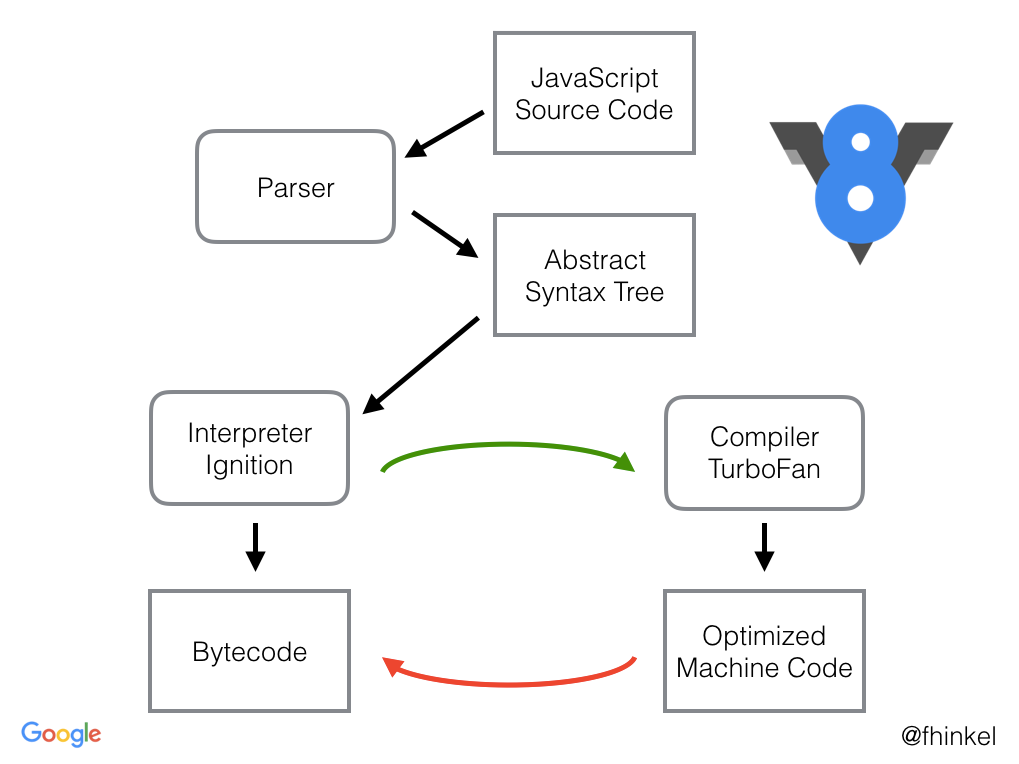
\includegraphics[width=0.6\textwidth]{images/v8-diagram.png}
        \caption{V8 Pipeline Diagram, from Franziska Hinkelmann's \href{https://medium.com/dailyjs/understanding-v8s-bytecode-317d46c94775}{\color{pink}``Understanding V8's Bytecode"}}
    \end{figure}
    \note{
        \begin{itemize}
            \item This diagram is simplified, and from 2017. Notably it does not contain Maglev.
            \item In late 2023 the V8 developers merged the early compiler, Maglev, into mainline.
            \item Regardless of the nyumber of compilers, these process generally stays the same.
            \item All modern javascript engines use multiple stages of compilation now. All are JIT'ed as well.
        \end{itemize}
    }
\end{frame}

\begin{frame}{Ignition}{--print-bytecode}
    Ignition uses the AST from the parser as well as feedback from Turbofan to generate an optimized IL representation.
    \begin{columns}
        \begin{column}{0.5\textwidth}
            \usemintedstyle{vim}
            \inputminted{js}{code/print-bytecode.tex}
        \end{column}
        \begin{column}{0.5\textwidth}
            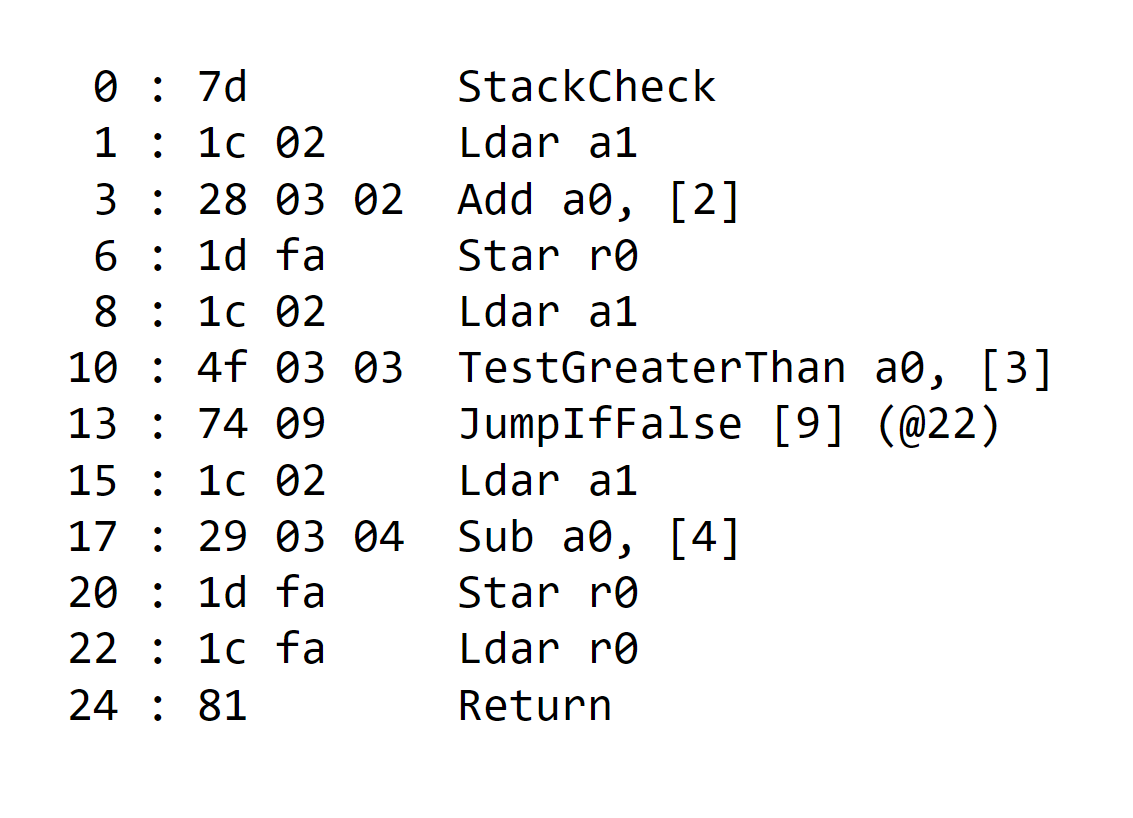
\includegraphics[width=\textwidth]{images/v8-ignition-bytecode.png}
        \end{column}
    \end{columns}
    \note{
        \begin{itemize}
            \item Note the flags to be run on d8, the v8 command line utility.
            \item ``Ldar" - Load Accumulator from register (a1, contains arg)
            \item ``Add"  - Add register ([2] is argument)
            \item ``Star" - Store accumulator into register ``result" into r0 
        \end{itemize}
    }
\end{frame}

\begin{frame}{Feedback into Ignition}{--allow-natives-syntax --print-opt-bytecode}
    \begin{columns}
        \begin{column}{0.5\textwidth}
            \usemintedstyle{vim}
            \inputminted{js}{code/ignition-feedback.tex}
        \end{column}
        \begin{column}{0.5\textwidth}
            \begin{itemize}
                \item  As a function runs, Turbofan will provide feedback to Ignition to generate more optimized bytecode. This includes type information, size information, and more! 
                \item Incorrect assumptions lead to a ``bailout" which leads to a de-optimization.
                \item This are lots of potential security problems here! The majority of vulnerabilities in V8 occur in the JIT engine!
            \end{itemize}
        \end{column}
    \end{columns}
    \note{
        \begin{itemize}
            \item The first loop contains the body of the function.  
            \item The second for loop contains code that makes the function ``hot" (able to be optimized).
            \item The \% sign is to force optimization, which must occur on ``hot" functions. \% functions require -allow-natives-syntax. 
            \item Finally, call the function forces the optimization process.
            \item The code here is ``dead" for integers, but is important for strings!
        \end{itemize}
    }
\end{frame}

\begin{frame}{Turbofan}{--allow-natives-syntax --trace-turbo}
    \begin{columns}
        \begin{column}{0.33\textwidth}
            \begin{itemize}
                \item Turbofan is the optimizing compiler of V8.
                \item It uses its ``Sea of Nodes" to generate a graph from the Ignition bytecode. 
                \item It also translates these nodes into machine code.
                \item Graphs can be visualized using \href{https://chromium.googlesource.com/v8/v8/+/refs/heads/main/tools/turbolizer/}{\color{pink}turbolizer}. 
            \end{itemize}
        \end{column}
        \begin{column}{0.67\textwidth}
            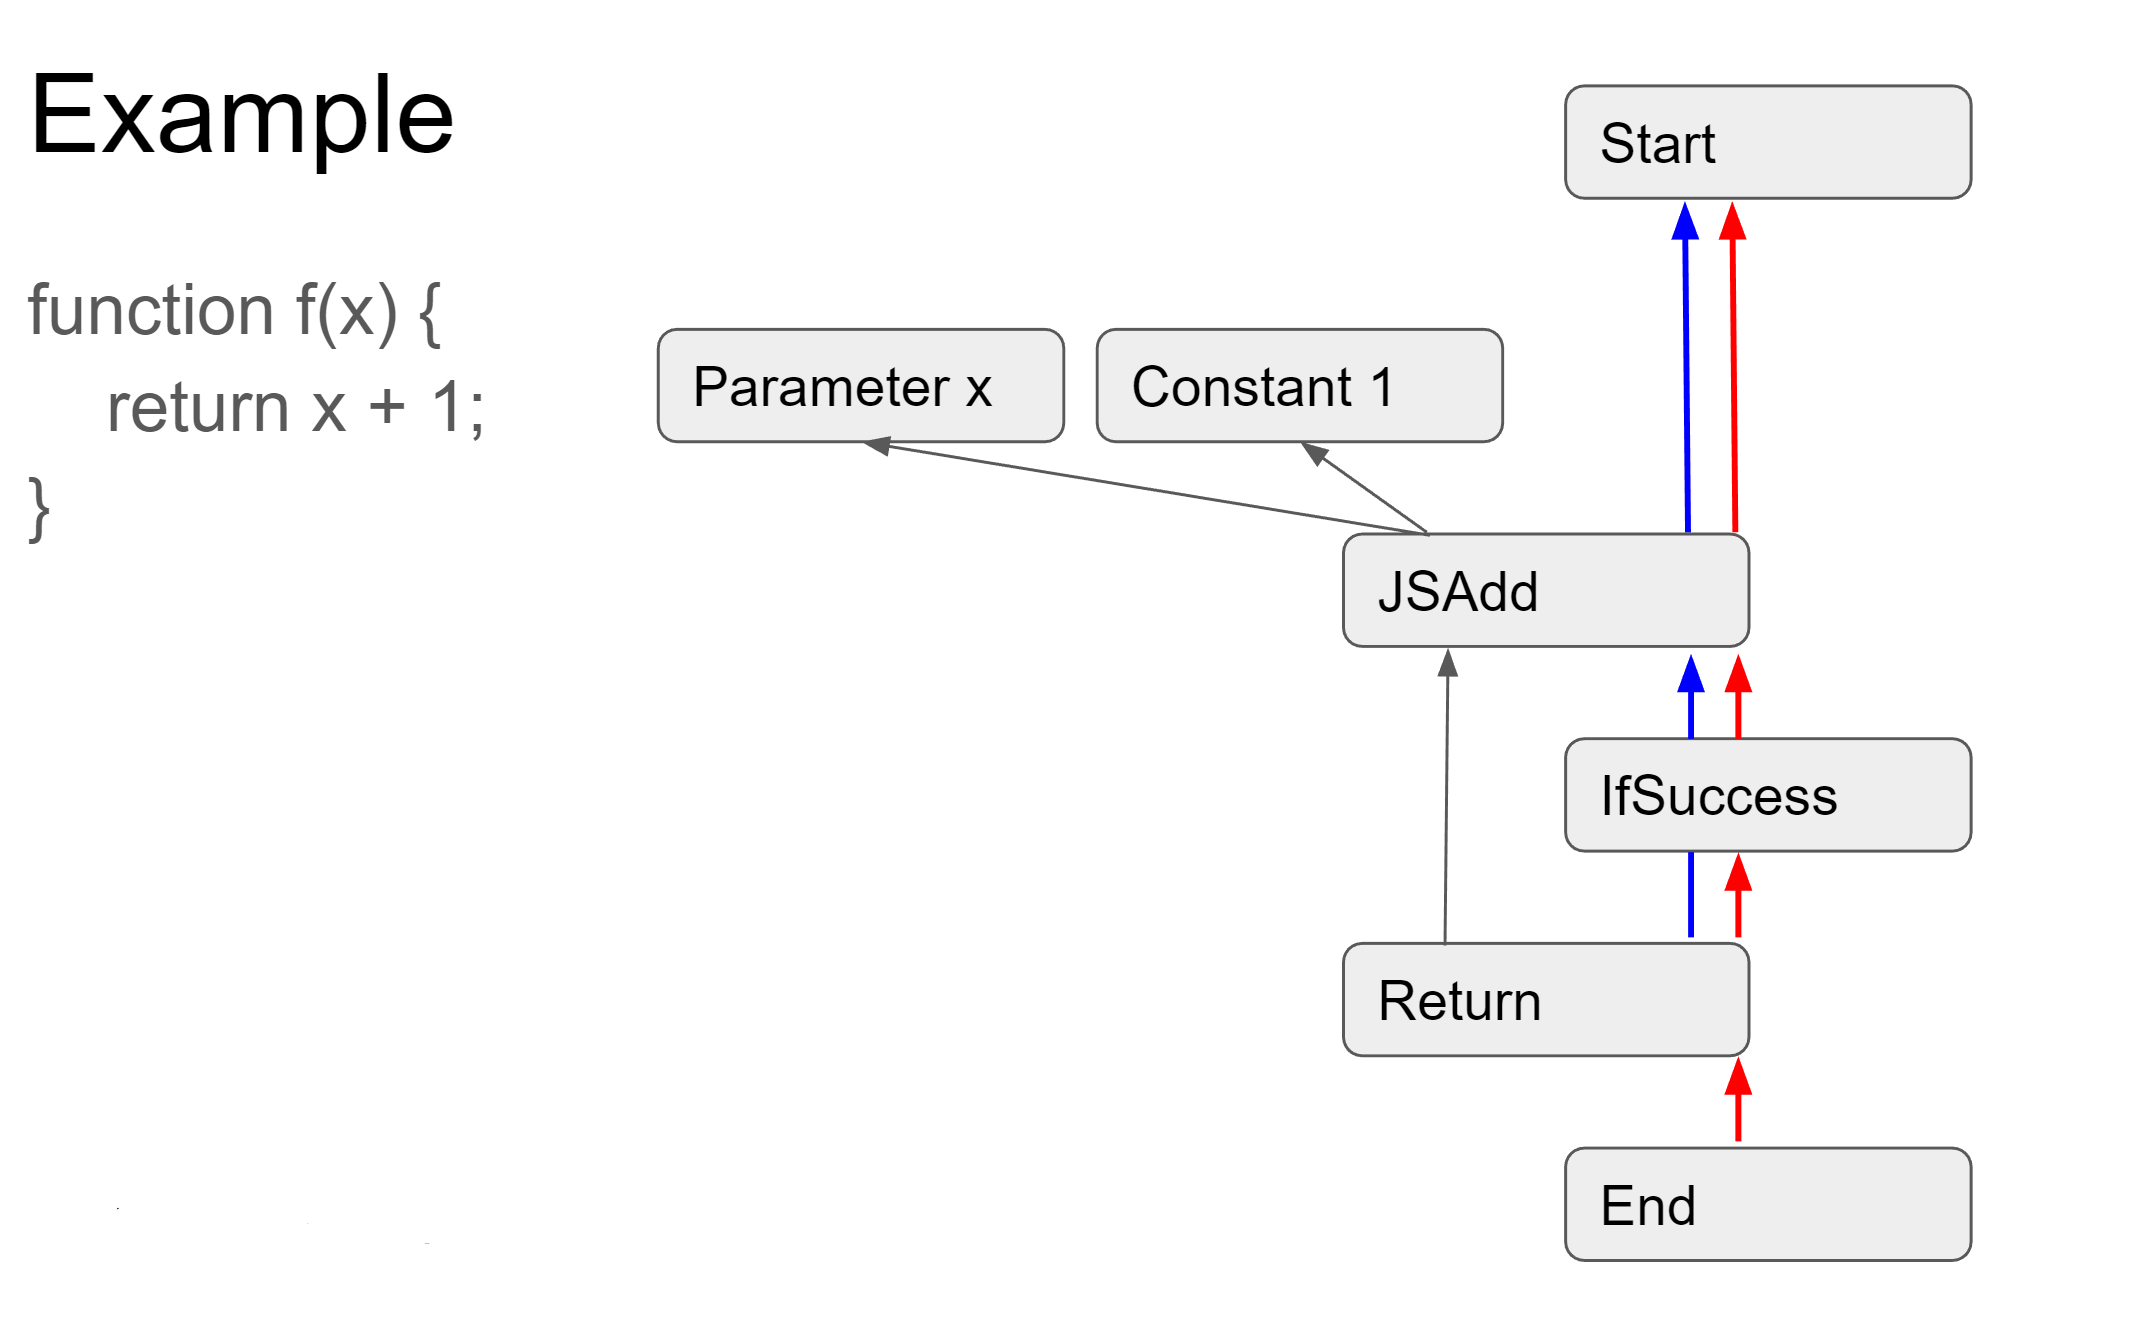
\includegraphics[width=\textwidth]{images/v8-basic-turbo-graph.png}
        \end{column}
    \end{columns}
    \note{
        \begin{itemize}
            \item Turbofan, historically, is the single largest source of exploitable bugs in the V8 engine.
            \item Note that while Turbofan is written in C++, most exploitable bugs in Turbofan and V8 are logical bugs.
            \item This means that a memory-safe implementation of Turbofan/V8 wouldn't really reduce exploitability much. 
        \end{itemize}
    }
\end{frame}

\begin{frame}{The V8 Pointer Cage}
    \begin{columns}
        \begin{column}{0.35\textwidth}
            \begin{itemize}
                \item Introduced in \href{https://v8.dev/blog/v8-release-92}{\color{pink}V8 v9.2}, the pointer cage is a namesake exploit protection employed by the V8 engine.
                \item Pointers in V8 are ``sandboxed" to never point outside of the JS Heap. 
                \item Modern pointers are all 32-bit and \textit{tagged} using \href{https://v8.dev/blog/pointer-compression}{\color{pink}pointer compression}.
            \end{itemize}
        \end{column}
        \begin{column}{0.65\textwidth}
            \begin{figure}
                \centering
                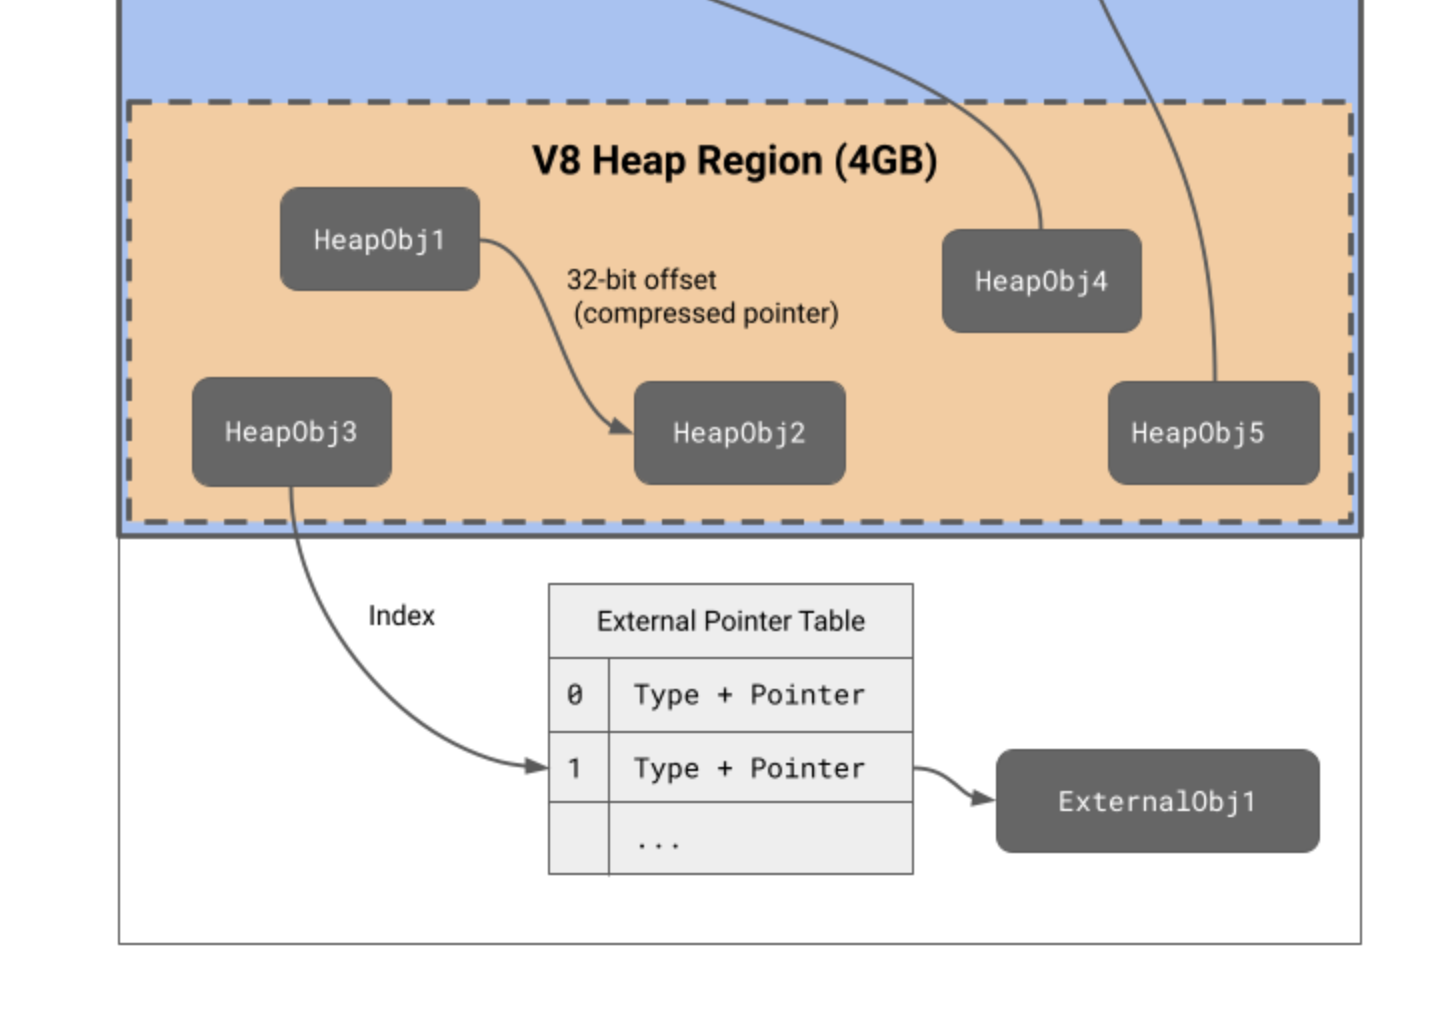
\includegraphics[width=0.80\textwidth]{images/v8-ptr-cage.png}
                \caption{The V8 memory layout with the pointer cage, from RAON.}
                \label{fig:v8-memory-layout}
            \end{figure}
        \end{column}
    \end{columns}
    \note{
        \begin{itemize}
            \item The V8 Pointer cage is the most prominent non-traditional exploit mitigation technique employed by the engine.
            \item Functionally, it eliminates pointers to valid memory addresses from anywhere inside of the heap where JavaScript objects are stored.
            \item Thus, if an attacker can leak memory back into JavaScript variables, they cannot leak pointers to valid memory addresses. 
            \item Tagged pointers are a concept in which the engine stores information about the pointer in its least significant bits.
            \item To do this, V8 assumes that all memory inside its engine is at least 4-byte aligned, giving it 2 bits of metadata it can use on any pointer. The glibc heap also does this.
            \item Other JS implementations use a technique called NaN-boxing, which abuses the IEEE 754 floating point structure.
        \end{itemize}
    }
\end{frame}